\documentclass[a4paper,11pt]{article}
\input{/home/tof/Documents/Cozy/latex-include/preambule_lua.tex}
\newcommand{\showprof}{show them}  % comment this line if you don't want to see todo environment
\fancyhead[L]{TP Sudoku}
\newdate{madate}{10}{09}{2020}
%\fancyhead[R]{\displaydate{madate}} %\today
%\fancyhead[R]{Seconde - SNT}
%\fancyhead[R]{Première - NSI}
\fancyhead[R]{Terminale - NSI}
\fancyfoot[L]{~\\Christophe Viroulaud}
\AtEndDocument{\label{lastpage}}
\fancyfoot[C]{\textbf{Page \thepage/\pageref{lastpage}}}
\fancyfoot[R]{\includegraphics[width=2cm,align=t]{/home/tof/Documents/Cozy/latex-include/cc.png}}
\usepackage{tikz}
\begin{document}
\begin{Form}
\section{Problématique}
Le Sudoku est un jeu aux règles simples mais qui offre un nombre de combinaisons énormes. Ainsi il existe $9!^9$ grilles possibles (soit $6 670 903 752 021 072 936 960$) qui correspond au nombre de façons de construire les régions sans tenir compte des contraintes sur les lignes et les colonnes. 
\begin{commentprof}
et encore plus de 5 milliards si on prend en compte un certains nombres de symétries, permutations...
\end{commentprof}
Il existe plusieurs variantes, mais les règle de base sont:
\begin{itemize}
\item chaque ligne ne contient qu'une série de chiffres de 1 à 9
\item chaque colonne ne contient qu'une série de chiffres de 1 à 9
\item chaque bloc ne contient qu'une série de chiffres de 1 à 9
\end{itemize}
\begin{center}
\shadowbox{\parbox{14cm}{\centering Peut-on créer un programme pour construire une grille complète et correcte?}}
\end{center}
\section{Modélisation}
Afin de simplifier le problème, concentrons-nous d'abord sur une grille de 4 de côté.
\begin{center}
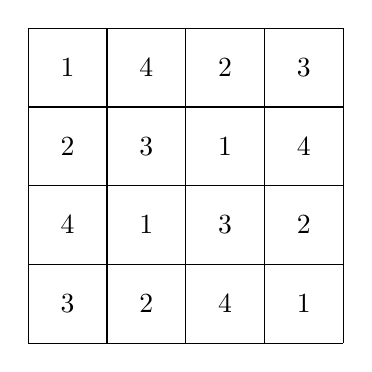
\begin{tikzpicture}
\draw (0,0) grid (4,4);
\node (00) at (0.5,0.5) {3};
\node (01) at (0.5,1.5) {4};
\node (02) at (0.5,2.5) {2};
\node (03) at (0.5,3.5) {1};

\node (10) at (1.5,0.5) {2};
\node (11) at (1.5,1.5) {1};
\node (12) at (1.5,2.5) {3};
\node (13) at (1.5,3.5) {4};

\node (20) at (2.5,0.5) {4};
\node (21) at (2.5,1.5) {3};
\node (22) at (2.5,2.5) {1};
\node (23) at (2.5,3.5) {2};

\node (30) at (3.5,0.5) {1};
\node (31) at (3.5,1.5) {2};
\node (32) at (3.5,2.5) {4};
\node (33) at (3.5,3.5) {3};

\end{tikzpicture}
\captionof{figure}{Grille 4×4}
\label{grille4}
\end{center}
Un graphe permet de modéliser les contraintes entre les cases. La figure \ref{grille4-2} ne montre que les arêtes qui partent de la case en haut à gauche. 
\begin{center}
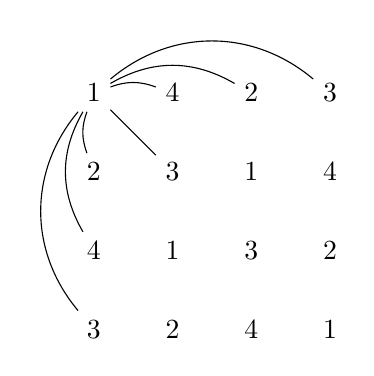
\begin{tikzpicture}
%\draw (0,0) grid (4,4);
\node (00) at (0.5,0.5) {3};
\node (01) at (0.5,1.5) {4};
\node (02) at (0.5,2.5) {2};
\node (03) at (0.5,3.5) {1};

\node (10) at (1.5,0.5) {2};
\node (11) at (1.5,1.5) {1};
\node (12) at (1.5,2.5) {3};
\node (13) at (1.5,3.5) {4};

\node (20) at (2.5,0.5) {4};
\node (21) at (2.5,1.5) {3};
\node (22) at (2.5,2.5) {1};
\node (23) at (2.5,3.5) {2};

\node (30) at (3.5,0.5) {1};
\node (31) at (3.5,1.5) {2};
\node (32) at (3.5,2.5) {4};
\node (33) at (3.5,3.5) {3};

\draw[-,>=latex] (03) to[bend right=20] (02);
\draw[-,>=latex] (03) to[bend right=30] (01);
\draw[-,>=latex] (03) to[bend right=40] (00);
\draw[-,>=latex] (03) to[bend left=20] (13);
\draw[-,>=latex] (03) to[bend left=30] (23);
\draw[-,>=latex] (03) to[bend left=40] (33);
\draw[-,>=latex] (03) to[bend left=0] (12);
\end{tikzpicture}
\captionof{figure}{Modélisation sous forme de graphe}
\label{grille4-2}
\end{center}
\section{Implémentation}
\subsection{Une classe Sudoku}
La classe \emph{Graphe} que nous avons déjà construite nous permettra de représenter les contraintes entre chaque case. Chaque sommet sera identifié par \emph{ses coordonnées dans la grille}. En parallèle nous utiliserons un tableau de tableaux pour contenir les chiffres à placer dans la grille.
\begin{center}
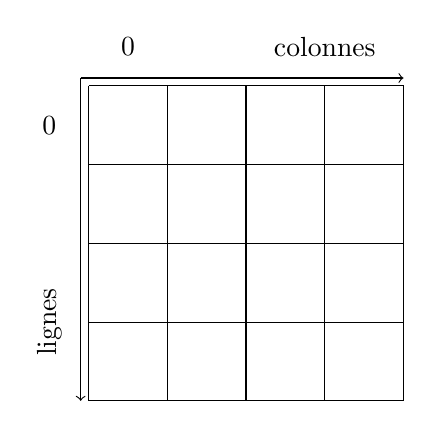
\begin{tikzpicture}
\draw (0,0) grid (4,4);
\draw[->] (-0.1,4.1) -- (-0.1,0);
\draw[->] (-0.1,4.1) -- (4,4.1);
\draw (-0.5,1)node[rotate=90]{lignes};
\draw (3,4.5)node{colonnes};
\draw (-0.5,3.5)node{0};
\draw (0.5,4.5)node{0};
\end{tikzpicture}
\captionof{figure}{Repérage des cases dans le système de coordonnées choisi.}
\label{coord}
\end{center}
\begin{activite}
Écrire la classe \emph{Sudoku} et son constructeur. Elle possédera trois attributs à initialiser:
\begin{itemize}
\item \textbf{taille: int} 4 pour un petit Sudoku,
\item \textbf{grille: list} à construire en fonction de la figure \ref{coord},
\item \textbf{graphe: Graphe}
\end{itemize}
\end{activite}
\subsection{Créer le graphe}
Comme le montre la figure \ref{grille4-2} chaque case doit respecter plusieurs contraintes. Ainsi nous procéderons en plusieurs étapes pour construire les arêtes:
\begin{itemize}
\item construire les sommets,
\item construire les arêtes verticales,
\item construire les arêtes horizontales,
\item construire les arêtes de blocs.
\end{itemize}
\begin{activite}
Écrire la méthode \textbf{creer\_graphe(self)$\;\rightarrow\;$None} qui construit le graphe.
\end{activite}
\subsection{Méthodes utiles}
Il est possible de parcourir le graphe de plusieurs manières. Puisque sa représentation est une grille carrée nous choisirons un balayage simple ligne par ligne.
\begin{activite}
Écrire la méthode \textbf{case\_suivante(self, s: tuple)$\;\rightarrow\;$tuple} qui renvoie les coordonnées, sous forme d'un tuple, de la case suivant celle de coordonnées \emph{s}.
\end{activite}
Pour chaque case à remplir, il faudra d'abord vérifier si le chiffre que l'on veut placer n'est pas déjà positionné sur une ligne, une colonne ou un bloc.
\begin{activite}
Écrire la méthode \textbf{est\_possible(self, s: tuple, choix: int)$\;\rightarrow\;$bool} qui renvoie \emph{True} si le chiffre \emph{choix} n'est pas déjà positionné dans une case \guill{adjacente} au sommet \emph{s}.
\end{activite}
\subsection{Remplir la grille}
Au départ, remplir la grille ne pose pas de difficultés car les choix sont nombreux. Cependant il peut apparaître rapidement des impossibilités. Il faut alors revenir en arrière, effacer les chiffres placés précédemment et recommencer. Cette description rapide montre un comportement récursif dans la méthodologie à adopter.\\
Formalisons cet algorithme:
\begin{itemize}
\item Si nous sortons de la grille, elle a été correctement remplie: renvoyer \emph{True}.
\item Sinon, pour chaque chiffre:
\begin{itemize}
\item S'il peut être positionné:
\begin{itemize}
\item Le placer dans la grille.
\item Remplir récursivement la case suivante et remonter \emph{True} dans la pile d'appel si le placement est correct.
\end{itemize}
\end{itemize}
Tous les chiffres ont été testés et aucun ne fonctionne: 
\item Réinitialiser la valeur de la case.
\item Remonter \emph{False} dans la pile d'appel.
\end{itemize}
\begin{activite}
Écrire la méthode \textbf{remplir\_rec(self, s: tuple = (0,0))$\;\rightarrow\;$None} qui implémente cet algorithme.
\end{activite}
\section{Affichage}
\begin{activite}
Écrire la méthode \textbf{afficher(self)$\;\rightarrow\;$None} qui utilise la bibliothèque \emph{tkinter} pour réaliser un affichage de la grille.
\end{activite}
\section{Aller plus loin}
\subsection{Construire une partie}
Partant d'un grille complète et correcte, il semble aisé de construire une partie. Il suffit de retirer aléatoirement des chiffres. Cependant des difficultés existent. En effet une partie est considérée correcte s'il n'existe qu'une seule solution. En enlevant des chiffres au hasard, nous pouvons sans le vouloir créer une partie qui aurait plusieurs issues.\\
Pire cela peut créer une situation bloquante où il devient impossible de compléter le jeu. L'expérience montre qu'il est possible de construire des jeux avec seulement 17 chiffres dévoilés. C'est d'ailleurs le nombre minimal d'indices que l'on peut donner. La preuve a été établie il y a quelques années comme le présente cet article du \emph{Monde}: \url{https://tinyurl.com/y4zmj4e7}.\\
En pratique à chaque retrait d'un chiffre, il faut vérifier que la partie est réalisable et la grille correcte.
\subsection{Résoudre une partie}
En modifiant légèrement la classe \emph{Sudoku}, il est possible de résoudre des parties rapidement. Il faut tout d'abord initialiser la grille avec les indices, puis modifier la fonction récursive pour qu'elle ne touche pas les cases fixées au départ.
\begin{figure}[!h]
\centering
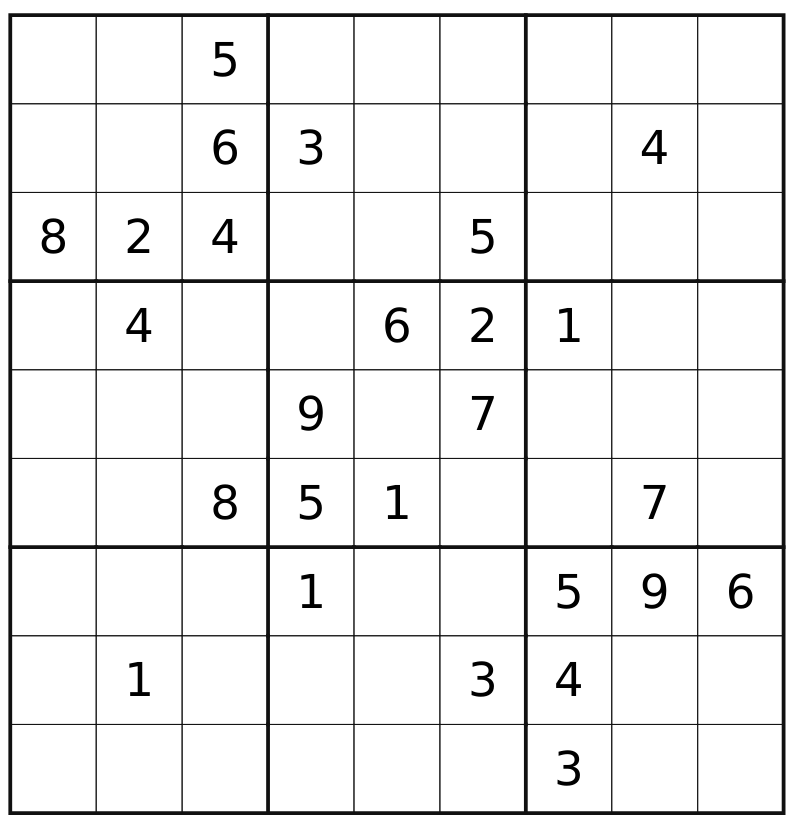
\includegraphics[width=5cm]{ressources/partie.png}
\captionof{figure}{À vous de jouer!}
\label{partie}
\end{figure}
\end{Form}
\end{document}